\documentclass{article}
\usepackage[backend=biber,natbib=true,style=alphabetic,maxbibnames=50]{biblatex}
\addbibresource{/home/nqbh/reference/bib.bib}
\usepackage[utf8]{vietnam}
\usepackage{tocloft}
\renewcommand{\cftsecleader}{\cftdotfill{\cftdotsep}}
\usepackage[colorlinks=true,linkcolor=blue,urlcolor=red,citecolor=magenta]{hyperref}
\usepackage{amsmath,amssymb,amsthm,enumitem,float,graphicx,mathtools,tikz}
\usetikzlibrary{angles,calc,intersections,matrix,patterns,quotes,shadings}
\allowdisplaybreaks
\newtheorem{assumption}{Assumption}
\newtheorem{baitoan}{Bài toán}
\newtheorem{cauhoi}{Câu hỏi}
\newtheorem{conjecture}{Conjecture}
\newtheorem{corollary}{Corollary}
\newtheorem{dangtoan}{Dạng toán}
\newtheorem{definition}{Definition}
\newtheorem{dinhly}{Định lý}
\newtheorem{dinhnghia}{Định nghĩa}
\newtheorem{example}{Example}
\newtheorem{ghichu}{Ghi chú}
\newtheorem{goal}{Goal}
\newtheorem{hequa}{Hệ quả}
\newtheorem{hypothesis}{Hypothesis}
\newtheorem{lemma}{Lemma}
\newtheorem{luuy}{Lưu ý}
\newtheorem{nhanxet}{Nhận xét}
\newtheorem{notation}{Notation}
\newtheorem{note}{Note}
\newtheorem{principle}{Principle}
\newtheorem{problem}{Problem}
\newtheorem{proposition}{Proposition}
\newtheorem{question}{Question}
\newtheorem{remark}{Remark}
\newtheorem{theorem}{Theorem}
\newtheorem{vidu}{Ví dụ}
\usepackage[left=1cm,right=1cm,top=5mm,bottom=5mm,footskip=4mm]{geometry}
\def\labelitemii{$\circ$}
\DeclareRobustCommand{\divby}{%
	\mathrel{\vbox{\baselineskip.65ex\lineskiplimit0pt\hbox{.}\hbox{.}\hbox{.}}}%
}
\setlist[itemize]{leftmargin=*}
\setlist[enumerate]{leftmargin=*}

\title{Lecture Note: Combinatorics {\it\&} Graph Theory\\Bài Giảng: Tổ Hợp {\it\&} Lý Thuyết Đồ Thị}
\author{Nguyễn Quản Bá Hồng\footnote{A scientist- {\it\&} creative artist wannabe, a mathematics {\it\&} computer science lecturer of Department of Artificial Intelligence {\it\&} Data Science (AIDS), School of Technology (SOT), UMT Trường Đại học Quản lý {\it\&} Công nghệ TP.HCM, Hồ Chí Minh City, Việt Nam.\\E-mail: {\sf nguyenquanbahong@gmail.com} {\it\&} {\sf hong.nguyenquanba@umt.edu.vn}. Website: \url{https://nqbh.github.io/}. GitHub: \url{https://github.com/NQBH}.}}
\date{\today}

\begin{document}
\maketitle
\begin{abstract}
	This text is a part of the series {\it Some Topics in Advanced STEM \& Beyond}:
	
	{\sc url}: \url{https://nqbh.github.io/advanced_STEM/}.
	
	Latest version:
	\begin{itemize}
		\item {\it Lecture Note: Combinatorics \& Graph Theory -- Bài Giảng: Tổ Hợp \& Lý Thuyết Đồ Thị}.
		
		PDF: {\sc url}: \url{https://github.com/NQBH/advanced_STEM_beyond/blob/main/combinatorics/lecture/NQBH_combinatorics_graph_theory_lecture.pdf}.
		
		\TeX: {\sc url}: \url{https://github.com/NQBH/advanced_STEM_beyond/blob/main/combinatorics/lecture/NQBH_combinatorics_graph_theory_lecture.tex}.
		\item {\it Slide: Combinatorics \& Graph Theory -- Slide Bài Giảng: Tổ Hợp \& Lý Thuyết Đồ Thị}.
		
		PDF: {\sc url}: \url{https://github.com/NQBH/advanced_STEM_beyond/blob/main/combinatorics/slide/NQBH_combinatorics_graph_theory_slide.pdf}.
		
		\TeX: {\sc url}: \url{https://github.com/NQBH/advanced_STEM_beyond/blob/main/combinatorics/slide/NQBH_combinatorics_graph_theory_slide.tex}.
		\item {\it Survey: Combinatorics \& Graph Theory -- Khảo Sát: Tổ Hợp \& Lý Thuyết Đồ Thị}.
		
		PDF: {\sc url}: \url{https://github.com/NQBH/advanced_STEM_beyond/blob/main/combinatorics/NQBH_combinatorics.pdf}.
		
		\TeX: {\sc url}: \url{https://github.com/NQBH/advanced_STEM_beyond/blob/main/combinatorics/NQBH_combinatorics.tex}.
		\item Codes:
		\begin{itemize}
			\item C{\tt/}C++: \url{https://github.com/NQBH/advanced_STEM_beyond/blob/main/combinatorics/C++}.
			\item Python: \url{https://github.com/NQBH/advanced_STEM_beyond/blob/main/combinatorics/Python}.
		\end{itemize}
	\end{itemize}
\end{abstract}
\tableofcontents

%------------------------------------------------------------------------------%

\section{Basic Combinatorics -- Tổ Hợp Cơ Bản}
Combinatorics is a collection of techniques \& a language for the study of (finite or countably infinite) discrete structures. Given a set of elements (\& possibly some structure on that set), typical questions in combinatorics are:
\begin{itemize}
	\item Does a specific arrangement of the elements exist?
	\item How many such arrangements are there?
	\item What properties do these arrangements have?
	\item Which 1 of the arrangements is maximal, minimal, or optimal according to some criterion?
\end{itemize}
-- Tổ hợp là một tập hợp các kỹ thuật \& một ngôn ngữ để nghiên cứu các cấu trúc rời rạc (hữu hạn hoặc vô hạn đếm được). Cho một tập hợp các phần tử (\& có thể có một số cấu trúc trên tập hợp đó), các câu hỏi điển hình trong tổ hợp là:
\begin{itemize}
	\item Có tồn tại sự sắp xếp cụ thể của các yếu tố không?
	\item Có bao nhiêu sự sắp xếp như vậy?
	\item Những sự sắp xếp này có những tính chất gì?
	\item Sự sắp xếp nào là tối đa, tối thiểu hoặc tối ưu theo một số tiêu chí?
\end{itemize}

%------------------------------------------------------------------------------%

\subsection{Notations}

\begin{itemize}
	\item $[n]\coloneqq\{1,2,\ldots,n\}$: the set of 1st $n\in\mathbb{N}^\star$ positive integers.
\end{itemize}

%------------------------------------------------------------------------------%

\subsection{Nguyên lý bù trừ}

\begin{dinhly}[Nguyên lý bù trừ{\tt/}nguyên lý bao hàm--loại trừ]
	\item(i) Với 2 tập hợp hữu hạn $A,B$ bất kỳ, $|A\cup B| = |A| + |B| - |A\cap B|$, $|A\backslash B| = |A| - |A\cap B|$.
	\item(ii) Với 3 tập hợp hữu hạn $A,B,C$ bất kỳ, $|A\cup B\cup C| = |A| + |B| + |C| - |A\cap B| - |B\cap C| - |C\cap A| + |A\cap B\cap C|$.
	\item(iii) Với $n\in\mathbb{N}^\star$, $A_i$, $i = 1,\ldots,n$, là $n$ tập hợp hữu hạn bất kỳ:
	\begin{equation*}
		\left|\bigcup_{i=1}^n A_i\right| = \sum_{T\subseteq\{1,\ldots,n\},\,T\ne\emptyset} (-1)^{|T| + 1}\left|\bigcap_{i\in T} A_i\right|.
	\end{equation*}
	Từ đó suy ra,
	\begin{equation*}
		\left|\bigcup_{i=1}^n A_i\right|\ge\sum_{i=1}^n |A_i| - \sum_{1\le i < j\le n} |A_i\cap A_j|.
	\end{equation*}
\end{dinhly}

%------------------------------------------------------------------------------%

\subsection{Method of mathematical induction \& recurrence -- Phương pháp quy nạp toán học \& truy hồi{\tt/}đệ quy}
{\sf Ideas of method of mathematical induction.} A sequence of {\it consecutive} pieces of domino falling.

-- {\sf Ý tưởng về phương pháp quy nạp toán học.} Một chuỗi các quân cờ domino {\it liên tiếp} rơi xuống.

{\sf Principle of Mathematical Induction.} Given an infinite sequence of propositions $\{P_n\}_{n=1}^\infty = P_1,P_2,\ldots,P_n,\ldots$, in order to prove that all of them are true, it is enough to show 2 things:
\begin{itemize}
	\item The base case: $P_1$ is true.
	\item The inductive step: For all $k\in\mathbb{N}^\star$, if $P_k$ is true, then so is $P_{k+1}$.
\end{itemize}

\begin{problem}[\cite{Shahriari2022}, p. 6]
	On a large square piece of paper, draw $n\in\mathbb{N}^\star$ straight lines that start from 1 side of the square \& end on another side. Each 2 of the lines intersect but no 3 (or more) lines go through the same point. Let $f(n)$ be the number of regions which the lines split the piece of paper. Compute some values of $f(n)$ \& predict its general formula.
\end{problem}

\begin{baitoan}[\cite{Shahriari2022}, p. 6]
	Trên một tờ giấy vuông lớn, vẽ $n\in\mathbb{N}^\star$ các đường thẳng bắt đầu từ 1 cạnh của hình vuông \& kết thúc ở cạnh còn lại. Mỗi 2 đường thẳng cắt nhau nhưng không có 3 (hoặc nhiều hơn) đường thẳng nào đi qua cùng một điểm. Giả sử $f(n)$ là số vùng mà các đường thẳng chia tờ giấy. Tính một số giá trị của $f(n)$ \& dự đoán công thức chung của nó.
\end{baitoan}

\begin{problem}[\cite{Shahriari2022}, p. 6]
	You have $100$ briefcases numbered $1$ through $100$. For any $n\in\mathbb{N}^\star$, if a briefcase numbered $n$ holds cash, then so does the briefcase numbered $n + 3$. You open up briefcase numbered $55$ \& it has a stuffed animal in it. Can you conclude anything about any of the other briefcases?
\end{problem}

\begin{baitoan}[\cite{Shahriari2022}, p. 6]
	Bạn có $100$ cặp được đánh số từ $1$ đến $100$. Đối với bất kỳ $n\in\mathbb{N}^\star$ nào, nếu một cặp được đánh số $n$ đựng tiền mặt, thì cặp được đánh số $n + 3$ cũng vậy. Bạn mở cặp được đánh số $55$ \& bên trong có một con thú nhồi bông. Bạn có thể kết luận điều gì về bất kỳ cặp nào khác không?	
\end{baitoan}

%------------------------------------------------------------------------------%

\subsection{Pigeonhole principle \& Ramsey theory -- Nguyên lý chuồng bồ câu \& lý thuyết Ramsey}

%------------------------------------------------------------------------------%

\subsection{Counting rules \& Stirling number of type 1 \& type 2}

\begin{problem}[\cite{Shahriari2022}, p. 2]
	Given $m,n\in\mathbb{N}^\star$, $m\le n$. Count the number of sequences $a_1,a_2,\ldots,a_n$ consisting of $m$ $0$'s \& $n - m$ $1$'s, if no 2 consecutive terms are both $0$'s?
\end{problem}

\begin{problem}[\cite{Shahriari2022}, p. 3]
	Let $f(n)$ be the number of subsets of $[n]$. Prove that $f(n) = 2^n$, $\forall n\in\mathbb{N}^\star$.
\end{problem}

\begin{problem}[\cite{Shahriari2022}, p. 3]
	Assume $n\in\mathbb{N}$, $n\ge2$, people given their $n$ hats to a hat-check person. Let $f(n)$ be the number of ways that the hats can be returned, so that everyone has 1 hat, but no one has their own hat. Prove: (a) $f(n) = n!\sum_{i=0}^n \dfrac{(-1)^i}{i!}$, $\forall n\in\mathbb{N}^\star$. (b) $f(n)$ is the nearest integer to $\dfrac{n!}{e}$.
\end{problem}

\begin{problem}[\cite{Shahriari2022}, p. 3]
	Given $n\in\mathbb{N}^\star$. Let $f(n)$ be the number of subsets of $[n]$ that do not contain 2 consecutive integers. (a) Compute $f(1),f(2),f(3),f(4)$. (b) Prove: $f(n) = f(n - 1) + f(n - 2)$, $\forall n\in\mathbb{N}$, $n\ge3$. (c) Prove:
	\begin{equation*}
		f(n) = \frac{1}{\sqrt{5}}\left(\tau^{n+2} - \overline{\tau}^{n+2}\right),\mbox{ where }\tau = \frac{1 + \sqrt{5}}{2},\ \overline{\tau} = \frac{1 - \sqrt{5}}{2}.
	\end{equation*}
\end{problem}

%------------------------------------------------------------------------------%

\subsection{Hoán vị \& tổ hợp}

\begin{baitoan}[Consecutive coin toss -- Gieo các đồng xu liên tiếp]
	Cho $n,k\in\mathbb{N}^\star$, $k\le n$. Tung 1 đồng xu đồng chất ngẫu nhiên $n$ lần. Tính xác suất lý thuyết của sự kiện: (a) Toàn bộ đều là mặt sấp (ngửa). (b) Có đúng $k$ lần xuất hiện mặt sấp (ngửa). (c) Có ít nhất $k$ lần xuất hiện mặt sấp (ngửa). (d) Có đúng $k$ lần xuất hiện mặt sấp (ngửa) liên tiếp nhau. (e) Có ít nhất $k$ lần xuất hiện mặt sấp (ngửa) liên tiếp nhau.
\end{baitoan}

\begin{proof}[Giải]
	Gọi $X_i\in\{S,N\}$ là biến cố ngẫu nhiên biểu diễn mặt đồng xu trong lần tung thứ $i$, $\forall i = 1,\ldots,n$. Không gian mẫu: $|\Omega| = \prod_{i=1}^n 2 = 2^n$. (a) Vì chỉ có 1 trường hợp thuận lợi là $(S,S,\ldots,S)$ nên $\mathbb{P}(X_i = S,\ \forall i = 1,\ldots,n) = \mathbb{P}(|\{i;X_i = S\}| = n) = \dfrac{1}{2^n}$. Tương tự, vì chỉ có 1 trường hợp thuận lợi là $(N,N,\ldots,N)$ nên $\mathbb{P}(X_i = N,\ \forall i = 1,\ldots,n) = \mathbb{P}(|\{i;X_i = N\}| = n) = \dfrac{1}{2^n}$. (b) $\mathbb{P}(|\{i;X_i = S\}| = k) = \mathbb{P}(|\{i;X_i = N\}| = k) = \dfrac{C_n^k}{2^n}$, $\forall k = 0,\ldots,n$. (c) $\mathbb{P}(|\{i;X_i = S\}|\ge k) = \mathbb{P}(|\{i;X_i = N\}|\ge k) = \dfrac{C_n^k + C_n^{k+1} + \cdots + C_n^n}{2^n} = \dfrac{\sum_{i=k}^n C_n^i}{2^n}$, $\forall k = 0,\ldots,n$. (d) $\mathbb{P} = \dfrac{n - k + 1}{2^n}$. (e) $\mathbb{P} = \dfrac{\sum_{i=k}^n (n - i + 1)}{2^n} = \dfrac{(n + 1)(n - k + 1) - \dfrac{(n + k)(n - k + 1)}{2}}{2^n}$.
	
\end{proof}

\begin{baitoan}[Simultaneous coin toss -- Gieo các đồng xu đồng thời]
	Cho $n,k\in\mathbb{N}^\star$, $k\le n$. Tung đồng thời $n$ đồng xu đồng chất ngẫu nhiên. Tính xác suất lý thuyết của sự kiện: (a) Toàn bộ đều là mặt sấp (ngửa). (b) Có đúng $k$ lần xuất hiện mặt sấp (ngửa). (c) Có ít nhất $k$ lần xuất hiện mặt sấp (ngửa).
\end{baitoan}

\begin{proof}[Giải]
	Gọi $X$ là biến cố ngẫu nhiên chỉ số mặt S xuất hiện khi tung đồng thời $n$ đồng xu. (a) $\mathbb{P}(X = n) = \mathbb{P}(X = 0) = \frac{1}{n + 1}$. (b) $\mathbb{P}(X = k) = \frac{1}{n + 1}$
\end{proof}

\begin{baitoan}[Consecutive 2 dice rolls -- Gieo 2 xúc xắc lần lượt]
	Gieo lần lượt 2 con xúc xắc. Tính xác suất lý thuyết của sự kiện: (a) 2 mặt có cùng số chấm, khác số chấm. (b) Số chấm 2 mặt có cùng tính chẵn lẻ, khác tính chẵn lẻ. (c) Số chấm 2 mặt đều là số nguyên tố, đều là hợp số, có ít nhất 1 số nguyên tố, có ít nhất 1 hợp số. (d) Số chấm 1 mặt là ước (bội) của số chấm trên mặt còn lại. (e) Tổng số chấm 2 mặt bằng $n\in\mathbb{N}$.
\end{baitoan}
{\sf Ans.} (e) $f(n) = (\min\{n - 1, 6\} - \max\{n - 6,1\} + 1){\bf1}_{n\in\{2,3,\ldots,12\}}$.

\begin{baitoan}[Simultaneous 2 dice rolls -- Gieo 2 xúc xắc đồng thời]
	Gieo đồng thời 2 con xúc xắc. Tính xác suất lý thuyết của sự kiện: (a) 2 mặt có cùng số chấm, khác số chấm. (b) Số chấm 2 mặt có cùng tính chẵn lẻ, khác tính chẵn lẻ. (c) Số chấm 2 mặt đều là số nguyên tố, đều là hợp số, có ít nhất 1 số nguyên tố, có ít nhất 1 hợp số. (d) Số chấm 1 mặt là ước (bội) của số chấm trên mặt còn lại. (e) Tổng số chấm 2 mặt bằng $n\in\mathbb{N}$.
\end{baitoan}

\begin{baitoan}[Consecutive $n$ dice rolls -- Gieo $n$ xúc xắc lần lượt]
	Gieo lần lượt $n\in\mathbb{N}^\star$ con xúc xắc. Tính xác suất lý thuyết của sự kiện: (a) $n$ mặt có cùng số chấm. (b) $n$ mặt có khác số chấm. (c) Số chấm $n$ mặt có cùng tính chẵn lẻ. (d) Số chấm 1 mặt là ước (bội) của số chấm trên các mặt còn lại. (e) Tổng số chấm $n$ mặt bằng $a\in\mathbb{N}$.
\end{baitoan}

\begin{baitoan}[Simultaneous $n$ dice rolls -- Gieo $n$ xúc xắc đồng thời]
	Gieo đồng thời $n\in\mathbb{N}^\star$ con xúc xắc. Tính xác suất lý thuyết của sự kiện: (a) $n$ mặt có cùng số chấm. (b) $n$ mặt có khác số chấm. (c) Số chấm $n$ mặt có cùng tính chẵn lẻ. (d) Số chấm 1 mặt là ước (bội) của số chấm trên các mặt còn lại. (e) Tổng số chấm $n$ mặt bằng $a\in\mathbb{N}$.
\end{baitoan}

\begin{baitoan}[Squares \& rectangles with same perimeter -- Hình vuông \& hình chữ nhật cùng chu vi]
	Cho $n\in\mathbb{N}^\star$. Viết n thành tổng 2 số: $n = a + b$. Tính xác suất để $a,b$ cùng là độ dài cạnh của 1 hình vuông, xác suất để $a,b$ là độ dài 2 cạnh của 1 hình chữ nhật nếu: (a) $a,b\in\mathbb{N}^\star$. (b) $a,b\in\mathbb{N}$.
\end{baitoan}

\begin{baitoan}[Squares \& rectangles with same area -- hình vuông \& hình chữ nhật cùng diện tích]
	Cho $a\in\mathbb{N}^\star,a\ge2$ có phân tích thừa số nguyên tố $a = \prod_{i=1}^{n} p_i^{a_i} = p_1^{a_1}p_2^{a_2}\cdots p_n^{a_n}$ với $p_i$ là số nguyên tố, $a_i\in\mathbb{N}^\star$, $\forall i = 1,2,\ldots,n$. (a) Viết ngẫu nhiên a thành tích của 2 số: $a = bc$. Tính xác suất để $b,c$ là độ dài 2 cạnh của 1 hình chữ nhật, xác suất để $b,c$ cùng là độ dài cạnh của 1 hình vuông nếu: (i) $b,c\in\mathbb{N}$. (ii) $b,c\in\mathbb{Z}$. (b) Lấy ngẫu nhiên 2 số $b,c\in\mbox{\rm Ư}(a)$. Tính xác suất để phân số $\dfrac{b}{c}$: (i) tối giản. (ii) không tối giản.
\end{baitoan}

\begin{definition}[Prime-counting function]
	The {\rm prime-counting function} is the function counting the number of prime numbers less than or equal to some real number x, denoted by $\pi(x)\coloneqq|\{p\in\mathbb{N}^\star|p \mbox{ is a prime},\ p\le x\}|$.
\end{definition}

\begin{dinhnghia}[Hàm đếm số số nguyên tố]
	{\rm Hàm đếm số số nguyên tố} là hàm đếm số số nguyên tố nhỏ hơn hoặc bằng $x\in\mathbb{R}$, ký hiệu là $\pi(x)\coloneqq|\{p\in\mathbb{N}^\star|p \mbox{ là số nguyên tố},\ p\le x\}|$.
\end{dinhnghia}

\begin{baitoan}[Prime, composite -- số nguyên tố, hợp số]
	Cho $m,n,k\in\mathbb{N}^\star$. Đặt $A_n = \{1,2,\ldots,n\}$ là tập hợp $n$ số nguyên dương đầu tiên, $\forall n\in\mathbb{N}^\star$. (a) Lấy m số từ $A_n$. Tính xác suất để m số này cùng chẵn, cùng lẻ, có ít nhất 1 số chẵn, có ít nhất 1 số lẻ, có đúng k số chẵn, có đúng k số lẻ, có ít nhất k số chẵn, có ít nhất k số lẻ. (b) Lấy m số phân biệt từ $A_n$. Tính xác suất để m số này đều là số nguyên tố, đều là hợp số, có đúng k số nguyên tố, có đúng k hợp số, có ít nhất 1 số nguyên tố, có ít nhất 1 hợp số, có ít nhất k số nguyên tố, có ít nhất k hợp số. (c) Viết chương trình {\sf Pascal, Python C{\tt/}C++} để mô phỏng việc tính các xác suất đó.
\end{baitoan}

\begin{baitoan}[Odd, even -- chẵn, lẻ]
	Cho $a,b\in\mathbb{Z},a < b$, $n,k\in\mathbb{N}^\star,n\ge2,k\le n$. Đặt $A = [a,b]\cap\mathbb{Z} = \{a,a + 1,a + 2,\ldots,b - 1,b\}$. (a) Lấy 2 số từ tập A. Xét 2 trường hợp phân biệt, không nhất thiết phân biệt. Tính xác suất để 2 số này cùng tính chẵn lẻ, khác tính chẵn lẻ. (b) Lấy n số từ tập A. Tính xác suất để n số này đều chẵn, đều lẻ, cùng tính chẵn lẻ, có đúng k số chẵn, k số lẻ, có ít nhất k số chẵn, k số lẻ. (c) Viết chương trình {\sf Pascal, Python C{\tt/}C++} để mô phỏng việc tính các xác suất đó.
\end{baitoan}

\begin{baitoan}[VMC2024B4]
	(a) Đếm số cách chọn ra 3 viên gạch, mỗi viên từ 1 hàng trong $3\times5$ viên gạch xếp xen kẽ, sao cho không có 2 viên gạch nào được lấy ra nằm kề nhau (2 viên gạch được gọi là kề nhau nếu có chung 1 phần của 1 cạnh).
	\begin{figure}[H]
		\centering
		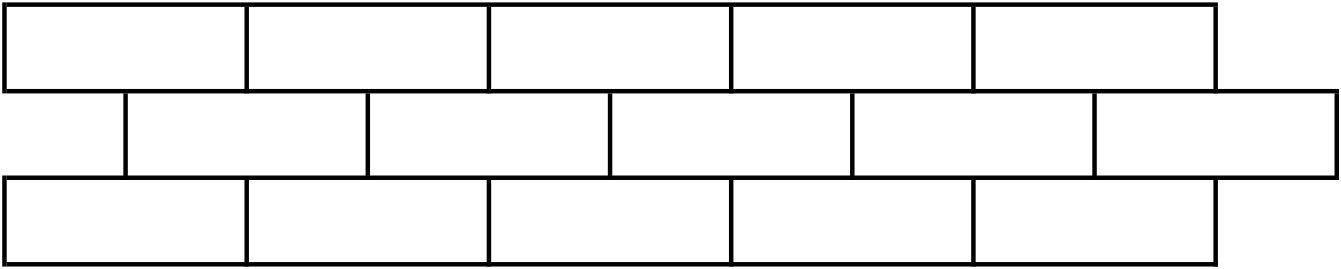
\includegraphics[width=8cm]{brick3x5}
	\end{figure}
	(b) Đếm số cách chọn ra 4 viên gạch, mỗi viên từ 1 hàng trong $4\times5$ viên gạch xếp xen kẽ, sao cho không có 2 viên gạch nào được lấy ra nằm kề nhau.
	\begin{figure}[H]
		\centering
		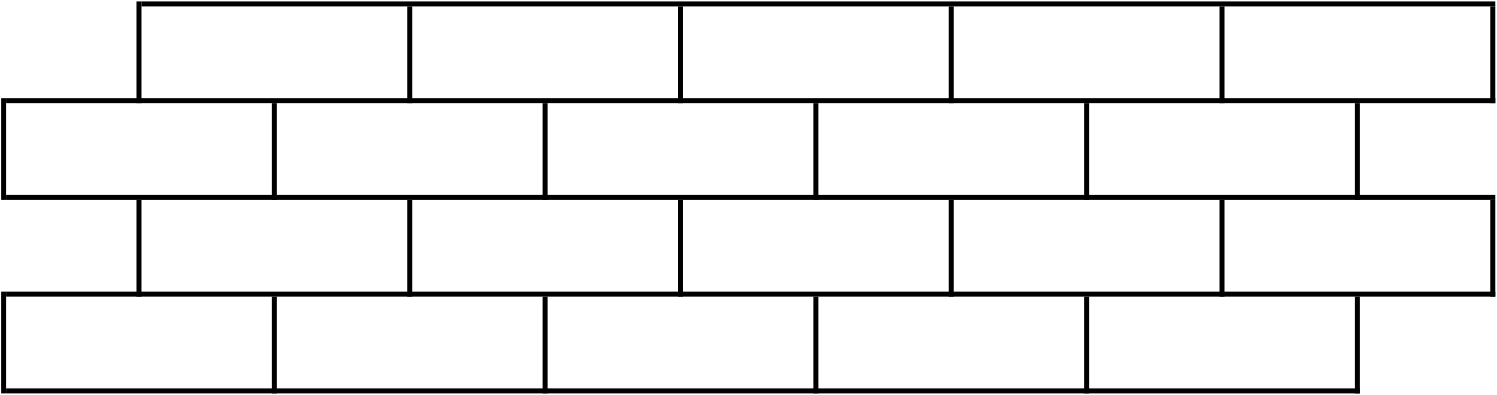
\includegraphics[width=8cm]{brick4x5}
	\end{figure}
	(c) Cho $m,n\in\mathbb{N}^\star$. Đếm số cách chọn ra $m$ viên gạch, mỗi viên từ 1 hàng trong $m\times n$ viên gạch xếp xen kẽ, sao cho không có 2 viên gạch nào được lấy ra nằm kề nhau. (d) Cho $m,n,k\in\mathbb{N}^\star$. Đếm số cách chọn ra $k$ viên gạch, không nhất thiết mỗi viên từ 1 hàng trong $m\times n$ viên gạch xếp xen kẽ, sao cho không có 2 viên gạch nào được lấy ra nằm kề nhau. (e${}^\star$) Mở rộng cho trường hợp $m\times n$ với số gạch mỗi hàng có thể khác nhau, cụ thể là hàng $i$ chứa $a_i\in\mathbb{N}^\star$ viên gạch, $\forall i = 1,\ldots,m$ với 2 trường hợp: (i) Mỗi viên từ 1 hàng. (ii) Lấy $k\in\mathbb{N}^\star$ viên gạch, mỗi hàng có thể lấy nhiều viên.
\end{baitoan}

\begin{nhanxet}[Left-right symmetry -- Đối xứng trái phải]
	Nếu số viên gạch của mỗi hàng bằng nhau \& được sắp xen kẽ như (a) \& (b), thì thứ tự viên gạch đầu tiên từ bên trái của mỗi hàng lồi ra hay thụt vào không quan trọng, vì có thể lấy đối xứng gương trái--phải để chuyển đổi 2 trường hợp đó. Cũng chú ý đến tính đối xứng trên--dưới (top-bottom symmetry).
\end{nhanxet}

\begin{proof}
	Số cách chọn gạch từ 3 hàng, mỗi hàng $n$ viên gạch: $(n - 1)(n - 2)^2 + (n - 1)^2 = (n - 1)(n^2 - 3n + 3)$, $\forall n\in\mathbb{N}^\star$, $n\ge2$. Số cách chọn gạch từ 4 hàng, mỗi hàng $n\in\mathbb{N}^\star$ viên gạch: $(n^2 - 3n + 3)^2$, $\forall n\in\mathbb{N}^\star$, $n\ge2$.
\end{proof}

\begin{itemize}
	\item C++ codes:
	\begin{itemize}
		\item (DKAK): \url{https://github.com/NQBH/advanced_STEM_beyond/blob/main/VMC/C++/brick_DPAK.cpp}.
		\item (NLDK): \url{https://github.com/NQBH/advanced_STEM_beyond/blob/main/VMC/C++/brick_NLDK.cpp}.
	\end{itemize}
\end{itemize}

%------------------------------------------------------------------------------%

\subsection{Hệ số nhị thức \& đa thức}

%------------------------------------------------------------------------------%

\subsection{Phân vùng số nguyên \& nguyên tắc loại suy}

%------------------------------------------------------------------------------%

\subsection{Generating function -- Hàm sinh}
{\bf Idea of generating functions.} If we want to find a formula for some function $f(n)$ with $n\in\mathbb{N}$, then we can form the generating function of $f(n)$:
\begin{equation}
	\label{generating function}
	\tag{genf}
	F(x)\coloneqq\sum_{n\ge0} f(n)x^n = f(0) + f(1)x + f(2)x^2 + \cdots + f(n)x^n + \cdots,
\end{equation}
so that $a_n$ is the coefficient of $x^n$ in the Taylor series expansion of $F(x)$ defined by \eqref{generating function}.

Here we are concerned with formal power series, \& questions of convergence do not come up (at least for elementary applications). Sometimes this power series has a nice closed form \& then we can manipulate this function \& get information about $f(n)$, $\forall n\in\mathbb{N}$.

-- Ở đây chúng ta quan tâm đến chuỗi lũy thừa chính thức, \& các câu hỏi về sự hội tụ không xuất hiện (ít nhất là đối với các ứng dụng cơ bản). Đôi khi chuỗi lũy thừa này có dạng đóng đẹp \& sau đó chúng ta có thể thao tác hàm này \& lấy thông tin về $f(n)$, $\forall n\in\mathbb{N}$.

\begin{problem}[\cite{Shahriari2022}, p. 4]
	Let $\{a_n\}_{n=0}^\infty$ be a sequence defined by
	\begin{equation*}
		a_0 = 1,\ \sum_{i=0}^n a_ia_{n-i} = 1,\ \forall n\in\mathbb{N}^\star.
	\end{equation*}
	(a) Let $F(x)\coloneqq\sum_{i=0}^\infty a_ix^i = a_0 + a_1x + a_2x^2 + \cdots$ be the generating function of $\{a_n\}_{n=0}^\infty$. Prove: $F(x)F(x) = \dfrac{1}{1 - x}$, thus $F(x) = \dfrac{1}{\sqrt{1 - x}}$. (b) Prove: $a_n = \dfrac{(2n - 1)!!}{2^nn!} = \dfrac{1\cdot3\cdot5\cdot(2n - 1)}{2^nn!}$, $\forall n\in\mathbb{N}^\star$.
\end{problem}

%------------------------------------------------------------------------------%

\section{Graph Theory -- Lý Thuyết Đồ Thị}
\textbf{\textsf{Resources -- Tài nguyên.}}
\begin{enumerate}
	\item \cite{Andreescu_Dospinescu2010}. {\sc Titu Andreescu, Gabriel Dospinescu}. {\it Problems From the Book}. Chap. 6: {\it Some Classical Problems in Extremal Graph Theory -- Vài Bài Toán Cổ Điển trong Lý Thuyết Đồ Thị Cực Trị}, pp. 119--136.
	
	\item \cite{Valiente2002, Valiente2021}. {\sc Gabriel Valiente}. {\it Algorithms on Trees \& Graphs With Python Code}. 2e.
\end{enumerate}

\subsection{Trees \& graphs: Some basic concepts -- Cây \& đồ thị: Vài khái niệm cơ bản}
The notion of graph which is most useful in computer science is that of a directed graph or just a graph. A graph is a combinatorial structure consisting of a finite nonempty set of objects, called vertices, together with a finite (possibly empty) set of ordered pairs of vertices, called directed edges or arcs.

-- Khái niệm đồ thị hữu ích nhất trong khoa học máy tính là đồ thị có hướng hoặc chỉ là đồ thị. Đồ thị là 1 cấu trúc tổ hợp bao gồm 1 tập hợp hữu hạn không rỗng các đối tượng, được gọi là các đỉnh, cùng với 1 tập hợp hữu hạn (có thể rỗng) các cặp đỉnh có thứ tự, được gọi là các cạnh có hướng hoặc cung.

\begin{definition}[Directed graph, \cite{Valiente2021}, Def. 1.1, p. 3]
	A {\rm graph} $G = (V,E)$ consists of a finite nonempty set $V$ of vertices \& a finite set $E\subseteq V\times V$ of edges. The {\rm order} of a graph $G = (V,E)$, denoted by $n$, is the number of vertices, $n = |V|$ \& the {\rm size}, denoted by $m$, is the number of edges, $m = |E|$. An edge $e = (v,w)$ is said to be {\rm incident} with vertices $v$ \& $w$, where $v$ is the {\rm source} \& $w$ the {\rm target} of edge $e$, \& vertices $v,w$ are said to be {\rm adjacent}. Edges $(u,v),(v,w)$ are said to be {\rm adjacent}, as are edges $(u,v),(w,v)$, \& also edges $(v,u),(v,w)$.
\end{definition}

\begin{dinhnghia}[Đồ thị có hướng]
	1 {\rm đồ thị} $G = (V,E)$ bao gồm 1 tập hữu hạn không rỗng $V$ các đỉnh \& 1 tập hữu hạn $E\subseteq V\times V$ các cạnh. {\rm Bậc} của 1 đồ thị $G = (V,E)$, ký hiệu là $n$, là số đỉnh, $n = |V|$ \& {\rm size}, ký hiệu là $m$, là số cạnh, $m = |E|$. Một cạnh $e = (v,w)$ được gọi là {\rm incident} với các đỉnh $v$ \& $w$, trong đó $v$ là {\rm source} \& $w$ {\rm target} của cạnh $e$, \& các đỉnh $v,w$ được gọi là {\rm kề}. Các cạnh $(u,v),(v,w)$ được gọi là {\rm kề}, cũng như các cạnh $(u,v),(w,v)$, \& cũng vậy các cạnh $(v,u),(v,w)$.
\end{dinhnghia}
Graphs are often drawn as a set of points in the plane \& a set of arrows, each of which joins 2 (not necessarily different) points. In a drawing of a graph $G = (V,E)$, each vertex $v\in V$ is drawn as a point or a small circle \& each edge $(v,w)\in E$ is drawn as an arrow from point or circle of vertex $v$ to the point or circle corresponding to vertex $w$.

-- Đồ thị thường được vẽ như một tập hợp các điểm trên mặt phẳng \& một tập hợp các mũi tên, mỗi mũi tên nối 2 điểm (không nhất thiết phải khác nhau). Trong bản vẽ đồ thị $G = (V,E)$, mỗi đỉnh $v\in V$ được vẽ như một điểm hoặc một đường tròn nhỏ \& mỗi cạnh $(v,w)\in E$ được vẽ như một mũi tên từ điểm hoặc đường tròn của đỉnh $v$ đến điểm hoặc đường tròn tương ứng với đỉnh $w$.

A vertex has 2 degrees in a graph, one given by the number of edges coming into the vertex \& the other given by the number of edges in the graph going out of the vertex.

-- Mỗi đỉnh có 2 bậc trong đồ thị, một bậc được xác định bởi số cạnh đi vào đỉnh \& bậc còn lại được xác định bởi số cạnh trong đồ thị đi ra khỏi đỉnh.

\begin{definition}[\cite{Valiente2021}, Def. 1.2, p. 4]
	The {\rm indegree} of a vertex $v$ in a graph $G = (V,E)$ is the number of edges in $G$ whose target is $v$, i.e., ${\rm indeg}(v) = |\{(u,v)|(u,v)\in E\}|$. The {\rm outdegree} of a vertex $v$ in a graph $G = (V,E)$ is the number of edges in $G$ whose source is $v$, i.e., ${\rm outdeg}(v) = |\{(v,w)|(v,w)\in E\}|$. The {\rm degree} of a vertex $v$ in a graph $G = (V,E)$ is the sum of the indegree \& the outdegree of the vertext, i.e., ${\rm deg}(v) = {\rm indeg}(v) + {\rm outdeg}(v)$.
\end{definition}
A basic relationship between the size of a graph \& the degree of its vertices, which will prove to be very useful in analyzing the computational complexity of algorithms on graphs:

-- Mối quan hệ cơ bản giữa kích thước của đồ thị \& bậc của các đỉnh, sẽ rất hữu ích trong việc phân tích độ phức tạp tính toán của các thuật toán trên đồ thị:

\begin{theorem}
	Let $G = (V,E)$ be a graph with $n$ vertices \& $m$ edges, \& let $V = \{v_1,\ldots,v_n\}$. Then
	\begin{equation*}
		\sum_{i=1}^n {\rm indeg}(v_i) = \sum_{i=1}^n {\rm outdeg}(v_i) = m.
	\end{equation*}
\end{theorem}
Walks, trails, \& paths in a graph are alternating sequences of vertices \& edges in the graph s.t. each edge in the sequence is preceded by its source vertex \& followed by its target vertex. Trails are walks having no repeated edges, \& paths are trails having no repeated vertices.

-- Đường đi, đường mòn, \& đường đi trong đồ thị là chuỗi xen kẽ các đỉnh \& cạnh trong đồ thị, tức là mỗi cạnh trong chuỗi được đi trước bởi đỉnh nguồn \& theo sau bởi đỉnh đích. Đường mòn là đường đi không có cạnh lặp lại, \& đường đi là đường mòn không có đỉnh lặp lại.

\begin{definition}[Walk, trail, path, \cite{Valiente2021}, Def. 1.3]
	A {\rm walk} from vertex $v_i$ to vertex $v_j$ in a graph is an alternating sequence $[v_i,e_{i+1},v_{i+1},e_{i+2},\ldots,v_{j-1},e_j,v_j]$ of vertices \& edges in the graph, s.t. $e_k = (v_{k-1},v_k)$ for $k = i + 1,\ldots,j$. A {\rm trail} is a walk with no repeated edges, \& a {\rm path} is a trail with no repeated vertices (except, possibly, the initial \& final vertices). The length of a walk, trail, or path is the number of edges in the sequence.
\end{definition}

\begin{dinhnghia}[Đường đi dạo, đường mòn, đường đi]
	1 {\rm đường đi dạo} từ đỉnh $v_i$ đến đỉnh $v_j$ trong một đồ thị là một chuỗi xen kẽ $[v_i,e_{i+1},v_{i+1},e_{i+2},\ldots,v_{j-1},e_j,v_j]$ các đỉnh \& cạnh trong đồ thị, s.t. $e_k = (v_{k-1},v_k)$ với $k = i + 1,\ldots,j$. Một {\rm đường mòn} là một cuộc đi bộ không có cạnh nào lặp lại, \& một {\rm đường đi} là một cuộc đi bộ không có đỉnh nào lặp lại (ngoại trừ, có thể là, các đỉnh đầu \& cuối). Độ dài của một cuộc đi bộ, trail hoặc path là số cạnh trong chuỗi.	
\end{dinhnghia}
Since an edge in a graph is uniquely determined by its source \& target vertices, a walk, trail, or path can be abbreviated by just enumerating either the vertices $[v_i,v_{i+1},\ldots,v_{j-1},v_j]$ or the edges $[e_{i+1},e_{i+2},\ldots,e_j]$ in the alternating sequence $[v_i,e_{i+1},v_{i+1},e_{i+2},\ldots,v_{j-1},e_j,v_j]$ of vertices \& edges.

-- Vì một cạnh trong đồ thị được xác định duy nhất bởi các đỉnh nguồn \& đích của nó, nên một đường đi, đường mòn hoặc đường dẫn có thể được rút gọn chỉ bằng cách liệt kê các đỉnh $[v_i,v_{i+1},\ldots,v_{j-1},v_j]$ hoặc các cạnh $[e_{i+1},e_{i+2},\ldots,e_j]$ trong chuỗi xen kẽ $[v_i,e_{i+1},v_{i+1},e_{i+2},\ldots,v_{j-1},e_j,v_j]$ các đỉnh \& cạnh.

Walks are closed if their initial \& final vertices coincide. -- Đường đi sẽ khép lại nếu đỉnh đầu \& đỉnh cuối trùng nhau.

\begin{definition}[Cycle, \cite{Valiente2021}, Def. 1.4]
	A walk, trail, or path $[v_i,e_{i+1},v_{i+1},e_{i+2},\ldots,v_{j-1},e_i,v_j]$ is said to be {\rm closed} if $v_i = v_j$. A {\rm cycle} is a closed path of length at least $1$.
\end{definition}
The combinatorial structure of a graph encompasses 2 notions of the substructure. A subgraph of a graph is just a graph whose vertex \& edge sets are contained in the vertex \& edge sets of the given graph, resp. The subgraph of a graph induced by a subset of its vertices has as edges the set of edges in the given graph whose source \& target belong to the subset of vertices.

-- Cấu trúc tổ hợp của một đồ thị bao gồm 2 khái niệm về cấu trúc con. Một đồ thị con của một đồ thị chỉ là một đồ thị có tập đỉnh \& cạnh được chứa trong tập đỉnh \& cạnh của đồ thị đã cho, tương ứng. Đồ thị con của một đồ thị được tạo ra bởi một tập con các đỉnh của nó có các cạnh là tập các cạnh trong đồ thị đã cho có nguồn \& đích thuộc về tập con các đỉnh.

\begin{definition}[Subgraph, \cite{Valiente2021}, Def. 1.5, p. 6]
	Let $G = (V,E)$ be a graph, \& let $W\subseteq V$. A graph $(W,S)$ is a {\rm subgraph} of $G$ if $S\subseteq E$. The subgraph of $G$ {\rm induced} by $W$ is the graph $(W,E\cap W\times W)$.
\end{definition}

\begin{dinhnghia}[Đồ thị con]
	Cho $G = (V,E)$ là một đồ thị, \& cho $W\subseteq V$. Một đồ thị $(W,S)$ là một {\rm đồ thị con} của $G$ nếu $S\subseteq E$. Đồ thị con của $G$ {\rm được tạo ra} bởi $W$ là đồ thị $(W,E\cap W\times W)$.
\end{dinhnghia}
The notion of graph which is most often found in mathematics is that of an undirected graph. Unlike the directed edges or edges of a graph, edges of an undirected graph have no direction association with them \& therefore, no distinction is made between the source \& target vertices of an edge. In a mathematical sense, an undirected graph consists of a set of vertices \& a finite set of undirected edges, where each edge has a set of 1 or 2 vertices associated with it. In the computer science view of undirected graphs, though, an undirected graph is the particular case of a directed graph in which for every edge $(v,w)$ of the graph, the reversed edge $(w,v)$ also belongs to the graph. Undirected graphs are also called {\it bidirected}.

-- Khái niệm đồ thị thường thấy nhất trong toán học là đồ thị vô hướng. Không giống như các cạnh hoặc cạnh có hướng của đồ thị, các cạnh của đồ thị vô hướng không có liên kết hướng nào với chúng \& do đó, không có sự phân biệt nào được tạo ra giữa các đỉnh nguồn \& đích của một cạnh. Theo nghĩa toán học, đồ thị vô hướng bao gồm một tập hợp các đỉnh \& một tập hợp hữu hạn các cạnh vô hướng, trong đó mỗi cạnh có một tập hợp gồm 1 hoặc 2 đỉnh được liên kết với nó. Tuy nhiên, theo quan điểm khoa học máy tính về đồ thị vô hướng, đồ thị vô hướng là trường hợp cụ thể của đồ thị có hướng trong đó đối với mọi cạnh $(v,w)$ của đồ thị, cạnh đảo ngược $(w,v)$ cũng thuộc về đồ thị. Đồ thị vô hướng cũng được gọi là {\it song hướng}.

\begin{definition}[Undirected graph, \cite{Valiente2021}, Def. 1.5, p. 6]
	A graph $G = (V,E)$ is {\rm undirected} if $(v,w)\in E\Rightarrow(w,v)\in E$, $\forall v,w\in V$.
\end{definition}

\begin{dinhnghia}[Đồ thị vô hướng]
	Đồ thị $G = (V,E)$ là {\rm vô hướng} nếu $(v,w)\in E\Rightarrow(w,v)\in E$, $\forall v,w\in V$.
\end{dinhnghia}


Denote by $d(V),C(V)$ the number, \& the set of vertices adjacent to a vertex $V$, respectively. A graph is said to have a {\it complete $k$-subgraph} if there are $k$ vertices any 2 of which are connected. A graph is said to be {\it $k$-free} if it does not contain a complete $k$-subgraph.

\begin{lemma}[\cite{Andreescu_Dospinescu2010}, Example 1, p. 121, Zarankiewicz's lemma]
	If $G$ is a $k$-free graph, then there exists a vertex having degree at most $\left\lfloor\dfrac{k - 2}{k - 1}n\right\rfloor$.
\end{lemma}
Zarankiewicz's lemma is the main step in the proof of Turan's theorem -- a famous classical result about $k$-free graphs.

\begin{theorem}[\cite{Andreescu_Dospinescu2010}, Example 2, p. 123, Turan's theorem]
	The greatest number of edges of a $k$-free graph with $n$ vertices is
	\begin{equation*}
		\frac{k - 2}{k - 1}\cdot\frac{n^2 - r^2}{2} + \binom{r}{2},
	\end{equation*}
	where $r$ is the remainder left by $n$ when divided to $k - 1$.
\end{theorem}

\begin{dinhnghia}[\cite{Ha_Thanh_to_hop}, Def. 7.2, p. 249, Đỉnh cô lập, lá]
	Cho $G$ là 1 đồ thị. Đỉnh có bậc $0$ được gọi là {\rm đỉnh cô lập}, đỉnh có bậc $1$ được gọi là {\rm lá}.
\end{dinhnghia}

\begin{dinhnghia}[\cite{Ha_Thanh_to_hop}, Def. 7.3, p. 249, Đồ thị chính quy]
	1 đồ thị được gọi là {\rm chính quy bậc $d$} hoặc {\rm$d$-chính quy} nếu mỗi đỉnh có bậc bằng $d\in\mathbb{N}$.
\end{dinhnghia}

\begin{dinhnghia}[\cite{Ha_Thanh_to_hop}, Def. 7.3, p. 249, Đỉnh thị khối]
	1 đồ thị được gọi là {\rm đồ thị bậc $3$} nếu nó chính quy bậc $3$, i.e., mỗi đỉnh đồ thị có bậc bằng $3$.
\end{dinhnghia}

\begin{goal}[Tính khả dĩ của dãy bậc của đồ thị]
	Tìm vài dấu hiệu hoặc vài điều kiện cần \& đủ để có thể quyết định liệu 1 dãy số nguyên dương $(a_i)_{i=1}^n\subset\mathbb{N}$ cho trươc có  thể thể là dãy bậc của đồ thị mà không phải vẽ biểu đồ.
\end{goal}

\begin{dinhnghia}[\cite{Ha_Thanh_to_hop}, Def. 7.6, p. 249, Dãy bậc của đồ thị, chuỗi đồ thị]
	{\rm Chuỗi bậc} của đồ thị là dãy bậc của các đỉnh của nó theo thứ tự không tăng. 1 dãy số nguyên không âm không tăng được gọi là {\rm đồ thị} nếu tồn tại 1 đồ thị có chuỗi bậc chính xác là dãy số nguyên không âm đó.
\end{dinhnghia}

\begin{vidu}[Sequence $1,1,\ldots,1$]
	$1,1,1$ không phải là 1 dãy đồ thị vì không thể xây dựng 1 đồ thị có 3 đỉnh sao cho tất cả 3 bậc là $1$. Nhưng $1,1$ \& $1,1,1,1$, hay nói chung các dãy chỉ toàn số $1$ với độ dài là 1 số chẵn, i.e., $\{1\}_{i=1}^{2n}$, $\forall n\in\mathbb{N}^\star$, là các dãy đồ thị, nhưng bất kỳ dãy chỉ toàn số $1$ với độ dài là 1 số lẻ, i.e., $\{1\}_{i=1}^{2n+1}$, $\forall n\in\mathbb{N}^\star$, thì không phải là 1 dãy đồ thị (why?)
\end{vidu}

\begin{dinhly}[Euler's, \cite{Ha_Thanh_to_hop}, Thm. 7.9, p. 250]
	\label{thm: Euler}
	Cho $G = (V,E)$ là đồ thị tổng quát với $d_1,\ldots,d_{|V|}\in\mathbb{N}$ là bậc của các đỉnh. Khi đó $\sum_{i=1}^{|V|} d_i = d_1 + d_2 + \cdots + d_{|V|} = 2|E|$. Nói riêng, số đỉnh của $G$ có bậc lẻ là số chẵn.
\end{dinhly}
Briefly:
\begin{equation*}
	d_1,\ldots,d_{|V|}\mbox{ are degrees of vertices of a graph } G = (V,E)\Rightarrow\sum_{i=1}^{|V|} d_i = 2|E|\Rightarrow|\{i;d_i\not{\divby}\ 2\}|\divby2.
\end{equation*}
Chú ý chiều ngược lại chưa chắc đúng:
\begin{vidu}
	Dãy số $7,5,5,4,3,2,2,0$ không mâu thuẫn với Định lý \ref{thm: Euler} nhưng nó không phải là đồ thị (why?).
\end{vidu}

\begin{question}
	Có thể suy ra được những hệ quả nào từ đẳng thức $\sum_{i=1}^{|V|} d_i = 2|E|$?
\end{question}

\begin{baitoan}
	Cho $G = (V,E)$ là đồ thị tổng quát với $d_1,\ldots,d_p\in\mathbb{N}$ là bậc của các đỉnh. Chứng minh: (i) Bậc cao nhất $d_{\max}\coloneqq\max_{1\le i\le p} d_i$ thỏa $d_{\max}\ge\dfrac{2|E|}{|V|}$. (ii)
\end{baitoan}

%------------------------------------------------------------------------------%

\section{CSES Problem Set{\tt/}Graph Algorithms}

\begin{problem}[CSES Problem Set{\tt/}counting rooms, \url{https://cses.fi/problemset/task/1192}]
	You are given a map of a building, \& your task is to count the number of its rooms. The size of the map is $n\times m$ squares, \& each square is either floor or wall. You can walk left, right, up, \& down through the floor squares.
	\item {\sf Input.} The 1st input lines has 2 integers $n,m$: the height \& width of the map. Then there are $n$ lines of $m$ characters describing the map. Each character is either . (floor) or {\tt\#} (wall).
	\item {\it Output.} Print 1 integer: the number of rooms.
	\item {\sf Constraints.} $1\le n,m\le10^3$.
	\item {\sf Sample.} Input:
	\begin{verbatim}
		5 8
		########
		#..#...#
		####.#.#
		#..#...#
		########		
	\end{verbatim}
	Output: {\tt3}.
\end{problem}

\begin{problem}[CSES Problem Set{\tt/}labyrinth, \url{https://cses.fi/problemset/task/1193}]
	You are given a map of a labyrinth, task: find a path from start to end. You can walk left, right, up, \& down.
	\item {\sf Input.} The 1st input line has 2 integers $n,m$: the height \& width of the map. Then there are $n$ lines $m$ characters describing the labyrinth. Each character is . (floor), {\tt\#} (wall), {\tt A} (start), or {\tt B} (end). There is exactly 1 {\tt A} \& 1 {\tt B} in the input.
	\item {\sf Output.} 1st print {\tt YES}, if there is a path, \& {\tt No} otherwise. If there is a path, print the length of the shortest such path \& its description as a string consisting of characters {\tt L} (left), {\tt R} (right), {\tt U} (up), \& {\tt D} (down). You can print any valid solution.
	\item {\sf Constraints.} $1\le n,m\le1000$.
	\item {\sf Sample.} Input:
	\begin{verbatim}
		5 8
		########
		#.A#...#
		#.##.#B#
		#......#
		########
	\end{verbatim}
	Output:
	\begin{verbatim}
		YES
		9
		LDDRRRRRU
	\end{verbatim}
\end{problem}

\begin{problem}[CSES Problem Set{\tt/}building roads, \url{https://cses.fi/problemset/task/1666}]
	Byteland has $n$ cities, \& $m$ roads between them. Goal: construct new roads so that there is a route between any 2 cities. Task: find out the minimum number of roads required, \& also determine which roads should be built.
	\item {\sf Input.} The 1st input line has 2 integers $n,m$: the number of cities \& roads. The cities are numbered $1,2,\ldots,n$. After that, there are $m$ lines describing the roads. Each lines has 2 integers $a,b$: there is a road between those cities. A road always connects 2 different cities, \& there is at most 1 road between any 2 cities.
	\item {\sf Output.} 1st print an integer $k$: the number of required roads. Then, print $k$ lines that describe the new roads. You can print any valid solution.
	\item {\sf Constraints.} $1\le n\le10^5,1\le m\le2\cdot10^5,1\le a,b\le n$.
	\item {\sf Sample.}
	\begin{table}[H]
		\centering
		\begin{tabular}{|l|l|}
			\hline
			\verb|build_road.inp| & \verb|build_road.out| \\
			\hline
			4 2 & 1 \\
			1 2 & 2 3 \\
			3 4 &  \\
			\hline
		\end{tabular}
	\end{table}
\end{problem}

\begin{problem}[CSES Problem Set{\tt/}message route, \url{https://cses.fi/problemset/task/1667}]
	Syrjälä's network has $n$ computers \& $m$ connections. Task: find out if Uolevi can send a message to Maija, \& if it is possible, what is the minimum number of computers on such a route.
	\item {\sf Input.} The 1st input line has 2 integers $n,m$: the number of computers \& connections. The computers are numbered $1,2,\ldots,n$. Uolevi's computer is $1$ \& Maija's computer is $n$. Then, there are $m$ lines describing the connections. Each line has 2 integers $a,b$: there is a connection between those computers. Every connection is between 2 different computers, \& there is at most 1 connection between any 2 computers.
	\item {\sf Output.} If it is possible to send a message, 1st print $k$: the minimum number of computers on a valid route. After this, print an example of such a route. You can print any valid solution. If there are no routes, print {\tt IMPOSSIBLE}.
	\item {\sf Constraints.} $2\le n\le10^5,1\le m\le2\cdot10^5,1\le a,b\le n$.
	\item {\sf Sample.}
	\begin{table}[H]
		\centering
		\begin{tabular}{|l|l|}
			\hline
			\verb|message_route.inp| & \verb|message_route.out| \\
			\hline
			5 5 & 3 \\
			1 2 & 1 4 5 \\
			1 3 & \\
			1 4 & \\
			2 3 & \\
			5 4 & \\
			\hline
		\end{tabular}
	\end{table}
\end{problem}

\begin{problem}[CSES Problem Set{\tt/}building team, \url{https://cses.fi/problemset/task/1668}]
	There are $n$ pupils in Uolevi's class, \& $m$ friendships between them. Task: divide pupils into 2 teams in such a way that no 2 pupils in a team are friends. You can freely choose the sizes of the teams.
	\item {\sf Input.} The 1st input line has 2 integers $n,m$: the number of pupils \& friendships. The pupils are numbered $1,2,\ldots,n$. Then, there are $m$ lines describing the friendships. Each line has 2 integers $a,b$: pupils $a,b$ are friends. Every friendship is between 2 different pupils. You can assume that there is at most 1 friendship between any 2 pupils.
	\item {\sf Output.} Print an example of how to build the teams. For each pupil, print {\tt1} or {\tt2} depending on to which team the pupil will be assigned. You can print any valid team. If there are no solutions, print {\tt IMPOSSIBLE}.
	\item {\sf Constraints.} $1\le n\le10^5,1\le m\le2\cdot10^5,1\le a,b\le n$.
	\item {\sf Sample.}
	\begin{table}[H]
		\centering
		\begin{tabular}{|l|l|}
			\hline
			\verb|build_team.inp| & \verb|build_team.out| \\
			\hline
			5 3 & 1 2 2 1 2 \\
			1 2 & \\
			1 3 & \\
			4 5 & \\
			\hline
		\end{tabular}
	\end{table}
\end{problem}

\begin{problem}[CSES Problem Set{\tt/}round trip, \url{https://cses.fi/problemset/task/1669}]
	Byteland has $n$ cities \& $m$ roads between them. Task: design a round trip that begins in a city, goes through 2 or more other cities, \& finally returns to starting city. Every intermediate city on the route has to be distinct.
	\item {\sf Input.} The 1st input line has 2 integers $n,m$: the number of cities \& roads. The cities are numbered $1,2,\ldots,n$. Then, there are $m$ lines describing the roads. Each line has 2 integers $a,b$: there is a road between those cities. Every road is between 2 different cities, \& there is at most 1 road between any 2 cities.
	\item {\sf Output.} 1st print an integer $k$: the number of cities on the route. Then print $k$ cities in order they will be visited. You can print any valid solution. If there are no solutions, print {\tt IMPOSSIBLE}.
	\item {\sf Constraints.} $1\le n\le10^5,1\le m\le2\cdot10^5,1\le a,b\le n$.
	\item {\sf Sample.}
	\begin{table}[H]
		\centering
		\begin{tabular}{|l|l|}
			\hline
			\verb|build_team.inp| & \verb|build_team.out| \\
			\hline
			5 6 & 4 \\
			1 3 & 3 5 1 3 \\
			1 2 & \\
			5 3 & \\
			1 5 & \\
			2 4 & \\
			4 5 & \\
			\hline
		\end{tabular}
	\end{table}
\end{problem}

\begin{problem}[CSES Problem Set{\tt/}monsters, \url{https://cses.fi/problemset/task/1194}]
	You \& some monsters are in a labyrinth. When taking a step to some direction in the labyrinth, each monster may simultaneously take 1 as well. Goal: reach 1 of the boundary squares without ever sharing a square with a monster. Task: find out if your goal is possible, \& if it is, print a path that you can follow. Your plan has to work in any situation; even if the monsters know your path beforehand.
	\item {\sf Input.} The 1st input line has 2 integers $n,m$: the height \& width of the map. After this there are $n$ lines of $m$ characters describing the map. Each character is . (floor), {\tt\#} (wall), {\tt A} (start), or {\tt M} (monster). There is exactly 1 {\tt A} in the input.
	\item {\sf Output.} 1st print {\tt YES} if your goal is possible, \& {\tt NO} otherwise. If your goal is possible, also print an example of a valid path (the length of the path \& its description using characters {\tt D, U, L, R}). You can print any path, as long as its length is at most $mn$ steps.
	\item {\sf Constraints.} $1\le m,n\le10^3$.
	\item {\sf Sample.} Input:
	\begin{verbatim}
		5 8
		########
		#M..A..#
		#.#.M#.#
		#M#..#..
		#.######
	\end{verbatim}
	Output:
	\begin{verbatim}
		YES
		5
		RRDDR
	\end{verbatim}
\end{problem}

\begin{problem}[CSES Problem Set{\tt/}shortest routes I, \url{https://cses.fi/problemset/task/1671}]
	There are $n$ cities \& $m$ flight connections between them. Task: determine the length of the shortest route from Syrjälä to every city.
	\item {\sf Input.} The 1st input line has 2 integers $n,m$: the number of cities \& flight connections. The cities are numbered $1,2,\ldots,n$, \& city $1$ is Syrjälä. After that, there are $m$ lines describing the flight connections. Each line has 3 integers $a,b,c$: a flight begins at city $a$, ends at city $b$, \& its length is $c$. Each flight is a 1-way flight. You can assume that it is possible to travel from Syrjälä to all other cities.
	\item {\sf Output.} Print $n$ integers: the shortest route lengths from Syrjälä to cities $1,2,\ldots,n$.
	\item {\sf Constraints.} $1\le n\le10^5,1\le m\le2\cdot10^5,1\le a,b\le n,1\le c\le10^9$.
	\item {\sf Sample.}
	\begin{table}[H]
		\centering
		\begin{tabular}{|l|l|}
			\hline
			\verb|shortest_route_I.inp| & \verb|shortest_route_I.out| \\
			\hline
			3 4 & 0 5 2 \\
			1 2 6 & \\
			1 3 2 & \\
			3 2 3 & \\
			1 3 4 & \\
			\hline
		\end{tabular}
	\end{table}
\end{problem}

\begin{problem}[CSES Problem Set{\tt/}shortest routes II, \url{https://cses.fi/problemset/task/1672}]
	There are $n$ cities \& $m$ roads between them. Task: process $q$ queries where you have to determine the length of the shortest route between 2 given cities.
	\item {\sf Input.} The 1st input line has 3 integers $n,m,q$: the number of cities, roads, \& queries. Then, there are $m$ lines describing the roads. Each line has 3 integers $a,b,c$: there is a road between cities $a$ \& $b$ whose length is $c$. All roads are 2-way roads. Finally, there are $q$ lines describing the queries. Each line has 2 integers $a,b$: determine the length of the shortest route between cities $a$ \& $b$.
	\item {\sf Output.} Print the length of the shortest route for each query. If there is no route, print {\tt-1} instead.
	\item {\sf Constraints.} $1\le n\le500,1\le m\le n^2,1\le q\le10^5,1\le a,b\le n,1\le c\le10^9$.
	\item {\sf Sample.}
	\begin{table}[H]
		\centering
		\begin{tabular}{|l|l|}
			\hline
			\verb|shortest_route_II.inp| & \verb|shortest_route_II.out| \\
			\hline
			4 3 5 & 5 \\
			1 2 5 & 5 \\
			1 3 9 & 8 \\
			2 3 3 & -1 \\
			1 2 & 3 \\
			2 1 & \\
			1 3 & \\
			1 4 & \\
			3 2 & \\
			\hline
		\end{tabular}
	\end{table}
\end{problem}

\begin{problem}[CSES Problem Set{\tt/}high score, \url{https://cses.fi/problemset/task/1673}]
	You play a game consisting of $n$ rooms \& $m$ tunnels. Your initial score is $0$, \& each tunnel increases your score by $x$ where $x$ may be both positive or negative. You may go through a tunnel several times. Task: walk from room $1$ to room $n$. What is the maximum score you can get?
	\item {\sf Input.} The 1st input line has 2 integers $n,m$: the number of rooms \& tunnels. The rooms are numbered $1,2,\ldots,n$. Then, there are $m$ lines describing the tunnels. Each line has 3 integers $a,b,x$: the tunnel starts at room $a$, ends at room $b$, \& it increases your score by $x$. All tunnels are 1-way tunnels. You can assume that it is possible to get from room $1$ to room $n$.
	\item {\sf Output.} Print 1 integer: the maximum score you can get. However, if you can get an arbitrarily large score, print {\tt-1}.
	\item {\sf Constraints.} $1\le n\le2500,1\le m\le5000,1\le a,b\le n,-10^9\le x\le10^9$.
	\item {\sf Sample.}
	\begin{table}[H]
		\centering
		\begin{tabular}{|l|l|}
			\hline
			\verb|high_score.inp| & \verb|high_score.out| \\
			\hline
			4 5 & 5 \\
			1 2 3 & \\
			2 4 -1 & \\
			1 3 -2 & \\
			3 4 7 & \\
			1 4 4 & \\
			\hline
		\end{tabular}
	\end{table}
\end{problem}

\begin{problem}[CSES Problem Set{\tt/}flight discount, \url{https://cses.fi/problemset/task/1195}]
	Task: find a minimum-price flight route from Syrjälä to Metsälä. You have 1 discount coupon, using which you can halve the price of any single flight during the route. However, you can only use the coupon once. When you use the discount coupon for a flight whose price is $x$, its price becomes $\lfloor\frac{x}{2}\rfloor$.
	\item {\sf Input.} The 1st input line has 2 integers $n,m$: the number of cities \& flight connections. The cities are numbered $1,2,\ldots,n$. City 1 is Syrjälä, \& city $n$ is Metsälä. After this there are $m$ lines describing the flights. Each line has 3 integers $a,b,c$: a flight begins at city $a$, ends at city $b$, \& its price is $c$. Each flight is unidirectional. You can assume that it is always possible to get from Syrjälä to Metsälä.
	\item {\sf Output.} Print 1 integer: the price of the cheapest route from Syrjälä to Metsälä.
	\item {\sf Constraints.} $1\le n\le10^5,1\le m\le2\cdot10^5,1\le a,b\le n,1\le c\le10^9$.
	\item {\sf Sample.}
	\begin{table}[H]
		\centering
		\begin{tabular}{|l|l|}
			\hline
			\verb|flight_discount.inp| & \verb|flight_discount.out| \\
			\hline
			3 4 & 2 \\
			1 2 3 & \\
			2 3 1 & \\
			1 3 7 & \\
			2 1 5 & \\
			\hline
		\end{tabular}
	\end{table}
\end{problem}

\begin{problem}[CSES Problem Set{\tt/}cycle finding, \url{https://cses.fi/problemset/task/1197}]
	You are given a directed graph, \& task: find out if it contains a negative cycle, \& also give an example of such a cycle.
	\item {\sf Input.} The 1st input line has 2 integers $n,m$: the number of nodes \& edges. The nodes are numbered $1,2,\ldots,n$. After this, the input has $m$ lines describing the edges. Each line has 3 integers $a,b,c$: there is an edge from node $a$ to node $b$ whose length is $c$.
	\item {\sf Output.} If the graph contains a negative cycle, print 1st {\tt YES}, \& then the nodes in the cycle in their correct order. If there are several negative cycles, you can print any of them. If there are no negative cycles, print {\tt NO}.
	\item {\sf Constraints.} $1\le n\le2500,1\le m\le5000,1\le a,b\le n,-10^9\le c\le10^9$.
	\item {\sf Sample.}
	\begin{table}[H]
		\centering
		\begin{tabular}{|l|l|}
			\hline
			\verb|cycle_finding.inp| & \verb|cycle_finding.out| \\
			\hline
			4 5 & YES \\
			1 2 1 & 1 2 4 1 \\
			2 4 1 & \\
			3 1 1 & \\
			4 1 -3 & \\
			4 3 -2 & \\
			\hline
		\end{tabular}
	\end{table}
\end{problem}

%------------------------------------------------------------------------------%

\section{CSES Problem Set{\tt/}Tree Algorithms}

%------------------------------------------------------------------------------%

\section{Posets, Kết Nối, Lưới Boolean}

%------------------------------------------------------------------------------%

\section{Miscellaneous}

%------------------------------------------------------------------------------%

\printbibliography[heading=bibintoc]
	
\end{document}